\documentclass[12pt,a4paper]{report}
%
% This LaTeX template has been created by Luca Grilli
% Based on the following https://en.wikibooks.org/wiki/LaTeX/Title_Creation
%
\usepackage[italian]{babel}
%\usepackage[T1]{fontenc} % Riga da commentare se si compila con PDFLaTeX
\usepackage{geometry}
\usepackage{graphicx}
\usepackage{hyperref}
\usepackage[utf8]{inputenc}
\usepackage{lipsum} % genera testo fittizio
\usepackage{subcaption}
\usepackage[nottoc,numbib]{tocbibind}
\usepackage{titlesec}

\titleformat{\chapter}[display]{\Huge\bfseries}{}{0pt}{\thechapter.\ }

\graphicspath{{figures/}}
%
%\addtolength{\topmargin}{-.875in} % reduce the default top margin
%\addtolength{\topmargin}{-2cm} % reduce the default top margin
%



%%%%%%%%%%%%%%%%%%%%%%%%%%%%%%%%%%
%                                %
%     Begin Docuemnt [start]     %
%                                %
%%%%%%%%%%%%%%%%%%%%%%%%%%%%%%%%%%
\begin{document}



%%%%%%%%%%%%%%%%%%%%%%%%%%%%%%
%     Title Page [start]     %
%%%%%%%%%%%%%%%%%%%%%%%%%%%%%%
% Declare new goemetry for the title page only.
\newgeometry{margin=1in}
\begin{titlepage}
	\centering
	
\includegraphics[width=0.30\textwidth]{logo-unipg}\par\vspace{1cm}
	\large{Presentazione Progetto di}\par
	\large{\textbf{Programmazione di Interfacce Grafiche e Dispositivi Mobili}}\par
	\small{Corso di Laurea in Ingegneria Informatica ed Elettronica -- A.A. 2019-2020}\par
	\textsc{\small{Dipartimento di Ingegneria}}\par

	%\vfill
	\vspace{0.5cm}
	docente\par
	Prof.~Luca \textsc{Grilli}

	\vspace{1cm}
	\vspace{1cm}
	\textbf{\huge{JPacman}}\par
	\vspace{0.2cm}
	applicazione desktop \textsc{JFC/Swing}\par
	\vspace{0.5cm}
	
\includegraphics[width=0.30\textwidth]{jpacman-icon}\par\vspace{1cm}
	\vspace{1cm}

	\large{studenti}\par
	\vspace{0.2cm}
	\begin{tabular}{ l l l l }
	\large{316649} & \large{\textbf{Francesca}} & \large{\textbf{Nocentini}} & \large{francesca.nocentini@studenti.unipg.it}\\
	\large{312294} & \large{\textbf{Paolo}} & \large{\textbf{Speziali}} & \large{paolo.speziali@studenti.unipg.it}\\
	\end{tabular}

	%\begin{tabular}{ l l l l }
	%112233 & Francesca & Nocentini & francesca.nocentini@studenti.unipg.it\\
	%114455 & Paolo & Speziali & paolo.speziali@studenti.unipg.it\\
	%\end{tabular}

	\vfill
	% Bottom of the page
	%{\large \today\par}
	\raggedright
	\small{Data ultimo aggiornamento: \today}
\end{titlepage}
% Ends the declared geometry for the titlepage
\restoregeometry
%%%%%%%%%%%%%%%%%%%%%%%%%%%%
%     Title Page [end]     %
%%%%%%%%%%%%%%%%%%%%%%%%%%%%

%%%%%%%%%%%%%%%%%%%%%%%%%%
%     Indice [start]     %
%%%%%%%%%%%%%%%%%%%%%%%%%%
\tableofcontents
%%%%%%%%%%%%%%%%%%%%%%%%
%     Indice [end]     %
%%%%%%%%%%%%%%%%%%%%%%%%

%%%%%%%%%%%%%%%%%%%%%%%%%%%%%%%%%%%%%%%%%%%%
%     Descrizione del Problema [start]     %
%%%%%%%%%%%%%%%%%%%%%%%%%%%%%%%%%%%%%%%%%%%%
\chapter{Descrizione del Problema}\label{ch:despro}
L'obiettivo di questo lavoro è lo sviluppo di un'applicazione desktop, denominata \emph{JPacman}, che realizza una versione graficamente e strutturalmente semplificata dell'omonimo videogioco di casa Namco~\cite{wiki:it:pacman,wiki:it:namco}.

L'applicazione sarà implementata utilizzando la tecnologia JFC/Swing in modo da favorire un'ampia portabilità su diversi sistemi operativi (piattaforme), riducendo al minimo eventuali modifiche al codice sorgente. Il codice prodotto sarà testato e ottimizzato per la piattaforma Windows 10.

%----------------------------------------------
% Sezione: Il Videogioco Arcade Pac-Man [start]
%----------------------------------------------
\section{Il Videogioco Arcade Pac-Man}\label{se:gal}
Il giocatore deve guidare una creatura sferica di colore giallo, chiamata Pac-Man, facendole mangiare tutti i numerosi puntini disseminati ordinatamente all'interno del labirinto e, nel far questo, deve evitare di farsi toccare da quattro fantasmi, che alternano la loro modalità Inseguimento (Chase) con quella di Spargimento (Scatter)~\cite{pacmanai}., pena la perdita immediata di una delle vite a disposizione. Per facilitare il compito al giocatore sono presenti, presso gli angoli dello schermo di gioco, quattro pillole speciali (\emph{PowerPills}) che rovesciano la situazione rendendo vulnerabili i fantasmi (modalità Frightened), che diventano blu e, per 10 secondi esatti, invertono la loro marcia; per guadagnare punti, è possibile in questa fase andare a caccia degli stessi fantasmi, per mangiarli.
Una volta fagocitati, però, questi tornano alla base (il rettangolo al centro dello schermo) sotto forma di un paio di occhi (modalità Eaten), per rigenerarsi e attaccare di nuovo Pac-Man. Completato un labirinto attraverso la fagocitazione di tutti i puntini, Pac-Man passa a quello successivo, identico nella struttura. I fantasmini hanno ognuno un comportamento differente nella modalità Chase:
\begin{itemize}
\item \textbf{Blinky} (Rosso): Il suo bersaglio è la posizione di Pac-Man;
\item \textbf{Pinky} (Rosa): Il suo bersaglio è quattro caselle di fronte a Pac-Man verso la direzione cui egli si sta muovendo;
\item \textbf{Inky} (Celeste): Il suo bersaglio è, preso come riferimento la lunghezza della linea che congiunge \textbf{Blinky} con la seconda casella di fronte a Pac-Man, l'estremità della linea lunga il doppio;
\item \textbf{Clyde} (Arancione): Il suo bersaglio è la posizione di Pac-Man finchè non si avvicina di 8 caselle, quando ciò avviene il suo bersaglio diventa quello della sua modalità Scatter;
\end{itemize}
Nella modalità Scatter i bersagli dei fantasmini sono quattro punti (uno per fantasma) posti ai lati del labirinto.

\begin{figure}[hb!]
\begin{subfigure}{.32\textwidth}
  \centering
  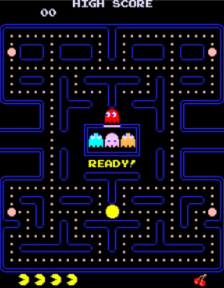
\includegraphics[width=.95\linewidth]{snapshot1}
  %\caption{1a}
  \caption{}
  \label{fig:snap1}
\end{subfigure}%
\begin{subfigure}{.32\textwidth}
  \centering
  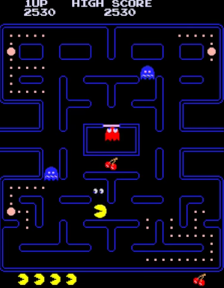
\includegraphics[width=.95\linewidth]{snapshot2}
  %\caption{1a}
  \caption{}
  \label{fig:snap2}
\end{subfigure}%
\begin{subfigure}{.32\textwidth}
  \centering
  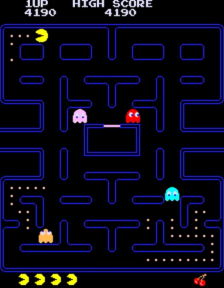
\includegraphics[width=.95\linewidth]{snapshot3}
  %\caption{1b}
  \caption{}
  \label{fig:snap3}
\end{subfigure}
\caption{Tre schermate del videogioco Pac-Man originale. La schermata (a) mostra l'inizio di una nuova partita. La schermata (b) mostra due fantasmi che scappano spaventati da Pac-Man dopo che questo ha mangiato una PowerPill, un fantasma rinato che torna all'inseguimento e un fantasma appena mangiato da Pac-Man che torna alla base. La schermata (c) mostra una partita quasi giunta alla conclusione.}
\label{fig:fig}
\end{figure}


%----------------------------------------------
% Sezione: Il Videogioco Arcade Pac-Man [end]
%----------------------------------------------



%----------------------------------------
% Sezione: L'applicazione JPacman [start]
%----------------------------------------
\section{L'applicazione JPacman}\label{se:appjgal}
L'applicazione JPacman replica in maniera fedele il gameplay del gioco originale.
I quattro fantasmi adottanno il comportamento classico Chase, Scatter, Frightened ed Eaten che era originariamente previsto, senza gli errori di movimento presenti nel cabinato originale (riferimento erroneamente spostato di alcune caselle se Pac-Man è rivolto verso l'alto). L'unica differenza dal gioco originale è la mancanza delle animazioni ``sketch" intermedie tra livelli.
%----------------------------------------
% Sezione: L'applicazione JPacman [end]
%----------------------------------------
%%%%%%%%%%%%%%%%%%%%%%%%%%%%%%%%%%%%%%%%%%
%     Descrizione del Problema [end]     %
%%%%%%%%%%%%%%%%%%%%%%%%%%%%%%%%%%%%%%%%%%



%%%%%%%%%%%%%%%%%%%%%%%%%%%%%%%%%%%%%%%%%%%
%     Specifica dei Requisiti [start]     %
%%%%%%%%%%%%%%%%%%%%%%%%%%%%%%%%%%%%%%%%%%%
%{\let\clearpage\relax \chapter{Specifica dei Requisiti}\label{ch:spereq}}
\chapter{Specifica dei Requisiti}\label{ch:spereq}

L'applicazione JPacman che si intende realizzare dovrà soddisfare i seguenti requisiti.

\begin{enumerate}
  \item Ricreare un labirinto in cui il personaggio e i nemici possano muoversi.
  \item Creare i quattro differenti nemici con i comportamenti del gioco originale (Chase/Scatter/Frightened/Eaten).
  \item Popolare il labirinto con le caratteristiche pillole e permettere al personaggio di raccoglierle ed accumulare punteggio.
  \item Popolare il labirinto con le caratteristiche PowerPill che permettono il passaggio alla modalità Frightened.
  \item Implementare un sistema di registrazione del punteggio.
  \item Implementazione delle animazioni di movimento e morte sia di Pac-Man che dei fantasmi.
  \item Popolare il labirinto con la caratteristica frutta per accumulare punteggio.
  \item Presenza di un sottofondo musicale e di effetti sonori attivabili/disattivabili dal pannello di configurazione dell’applicazione.
  \item Possibilità di metter in pausa il gioco con la pressione di un pulsante.
  \item Applicare un graduale aumento della difficoltà a seconda del livello raggiunto (fino ad un certo livello in cui si stabilizzerà).
  \item Arricchire il gioco con un movimento fluido dei personaggi all'interno del labirinto.
  \item Inserimento di due scenari (labirinti) extra.
  \item Inserimento dei tunnel di teletrasporto nei labirinti \textit{(facoltativo)}.
  \item Aggiunta di un editor di livelli che permetta al giocatore di crearne di nuovi \textit{(facoltativo)}.
\end{enumerate}
%%%%%%%%%%%%%%%%%%%%%%%%%%%%%%%%%%%%%%%%%
%     Specifica dei Requisiti [end]     %
%%%%%%%%%%%%%%%%%%%%%%%%%%%%%%%%%%%%%%%%%



%%%%%%%%%%%%%%%%%%%%%%%%%%%%
%     Progetto [start]     %
%%%%%%%%%%%%%%%%%%%%%%%%%%%%
\chapter{Progetto}\label{ch:prog}

% Architettura del Sistema Software [start]
%-------------------------------------------
\section{Architettura del Sistema Software}\label{ch:arch}
Nello sviluppo dell’applicazione siamo partiti con l'idea di sviluppare un gioco altamente modulare, che ci offrisse oggetti da poter riutilizzare senza troppe modifiche in altri ambiti e con funzionalità che potessero essere rimosse ed aggiunte all’occorrenza. Anziché seguire pattern come quello del Model-View-Controller abbiamo cercato di inglobare il comportamento di ogni entità all’interno di singole classi a sé stanti: ogni personaggio ed elemento dell’applicativo contiene infatti non solo le informazioni sul suo stato, la sua posizione e il frame dell’animazione, calcolato con un apposito oggetto, ma anche un Timer che gli permette di implementare un cambio dinamico dei suoi valori a seconda dei casi che gli vengono notificati.

Si è perciò arrivati allo sviluppo di un effettivo motore di gioco per videogame che implementano labirinti: poter creare un nuovo oggetto con cui interagire, un nuovo personaggio o addirittura un altro gioco, basandosi sulle strutture e le classi astratte da noi create, appare decisamente semplice una volta capita la logica di interazione. Sono poi presenti classi di supporto, come il gestore dei suoni e quello delle immagini memorizzate nel File System, classi che implementano KeyListener, ActionListener e classi che permettono la gestione delle animazioni con facilità (omesse dalla rappresentazione grafica riportata qui sopra).

A discapito potrebbe esserci la portabilità dell’applicazione su altri sistemi, tuttavia la modularità con cui è stata pensata e la gerarchia di classi permette una semplicità di sostituzione delle componenti che, secondo il nostro parere, non dovrebbe divergere poi molto da quella che si riscontra nelle applicazioni sviluppate con pattern Model-View-Controller.

L'idea di organizzare il codice in questo modo deriva dalla nostra personale esperienza e dall’osservazione della struttura di alcuni videogiochi che gestivano gli sprite e l’ambiente che li circondava in modo analogo.

\begin{figure}[bt]
  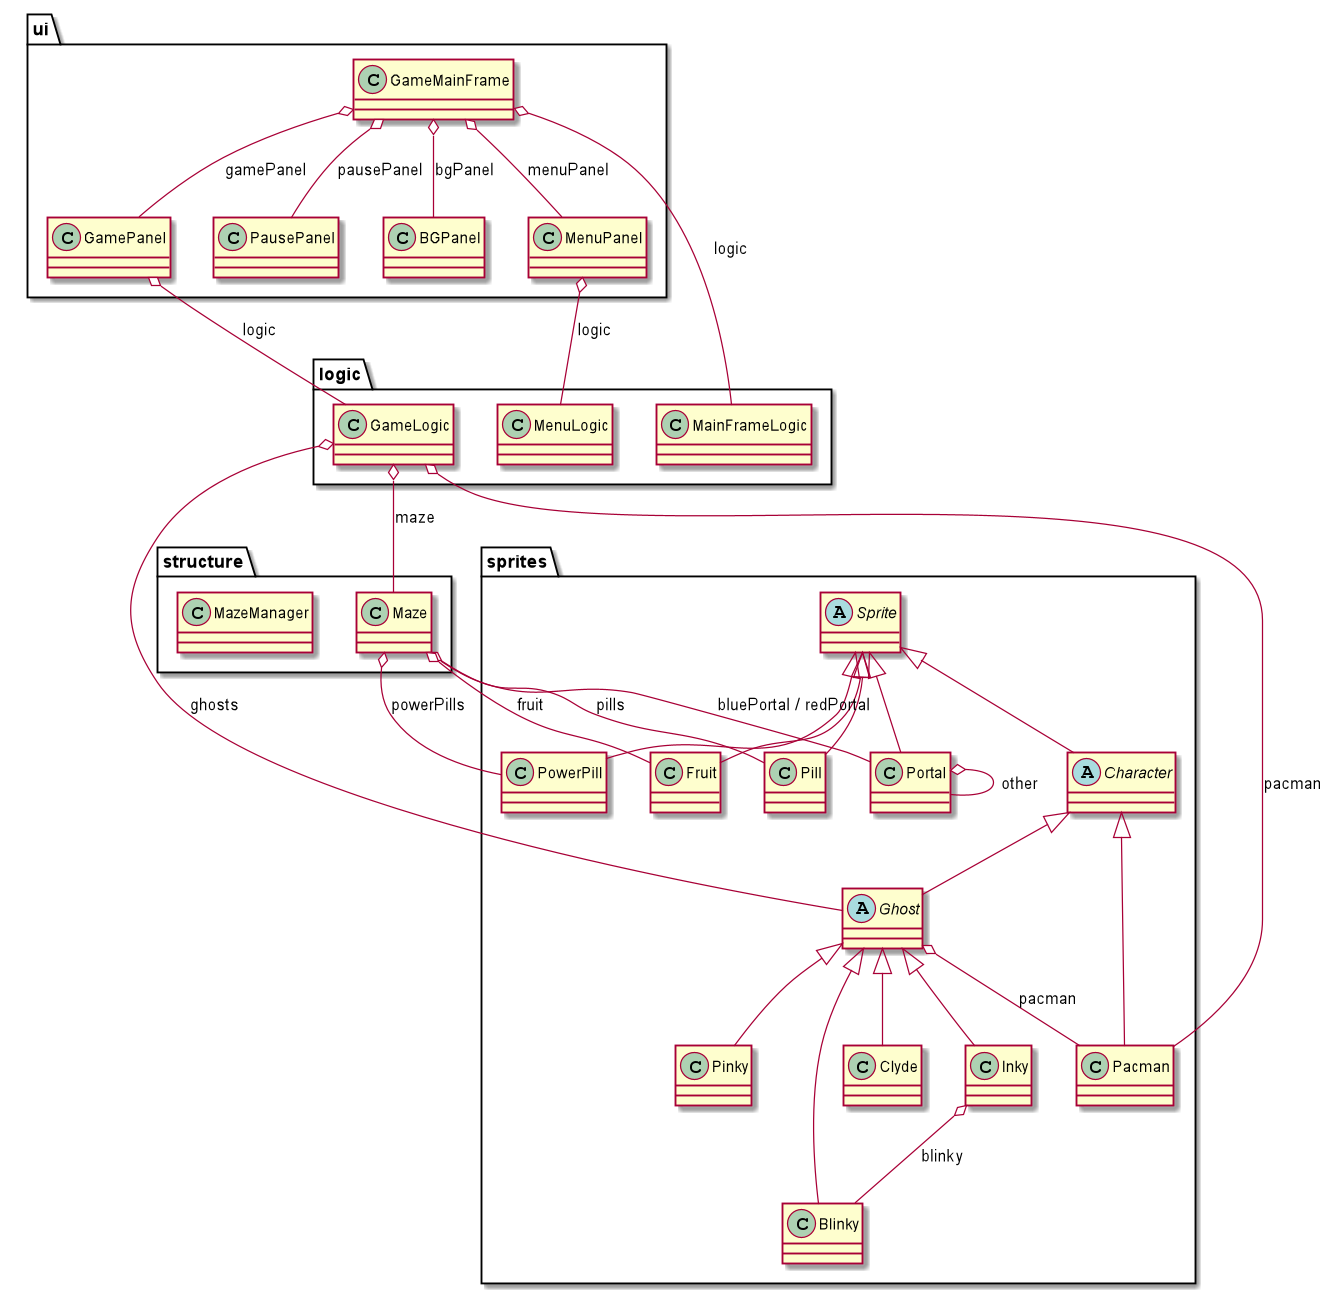
\includegraphics[width=.98\linewidth]{jpacman-UML}
\end{figure}

Possiamo osservare come la nostra applicazione sia composta da quattro moduli principali:
\begin{itemize}
 \item \textbf{UI} (User Interface): Classi che si occupano di stampare su schermo le componenti grafiche e gli oggetti immagine che gli vengono forniti. Le porzioni di codice comprese sono quasi esclusivamente finalizzate alla stampa e non comprendono logiche proprie di gioco.
 \item \textbf{Logic}: Classi controparti delle loro “omonime” della UI (es. GameLogic - GamePanel), contengono i metodi logici che scelgono cosa stampare e con quale criterio, definiscono quindi l’effettivo gameplay.
 \item \textbf{Sprites}: Classi che rappresentano entità tangibili su schermo, che siano personaggi o elementi di gioco, incapsulano tutte le informazioni che li riguardano (posizione, quantità di movimento progressivo, punto di nascita, frame della loro animazione, ecc…), che forniranno al Logic all’occorrenza. Inoltre, se sono Characters, mutano anche le loro caratteristiche in maniera dinamica (grazie all’ausilio delle classi del package loops).
 \item \textbf{Structure}: Permette la creazione dell’oggetto labirinto che gestisce tutti gli sprite statici che lo popolano e li fornisce al logic, inoltre offre metodi di supporto per i Characters in modo che possano muoversi nella struttura.\newpage
\end{itemize}


% Architettura del Sistema Software [end]
%-------------------------------------------

% UI [start]
%-------------------------------------------

\section{UI}\label{se:arch.ui}
In Fig.~\ref{fig:ui} viene illustrato il digramma di classe del modulo UI.\newline

Le classi facenti parte di questo package sono le uniche che, escludendo il riferimento alla loro immagine attuale degli sprite, operano con delle componenti grafiche e si occupano di stamparle su schermo. Eccetto GameMainFrame che estende JFrame, tutte estendono JPanel. Nel GameMainFrame infatti ci occuperemo di impilare questi quattro pannelli, con l’ausuilio di un JLayeredPane, a seconda delle necessità: mentre l’unico presente all’avvio sarà MenuPanel, che mostrerà appunto il menù principale, appena il gioco verrà avviato questo verrà sostituito da BGPanel, con la struttura del labirinto, con sopra GamePanel per mostrare gli sprite presenti in esso e le JLabel di stato. Alla pressione del tasto Invio sopra i due pannelli verrà posto PausePanel che mostrerà il menù di pausa con le sue opzioni.

\begin{figure}[tb]
  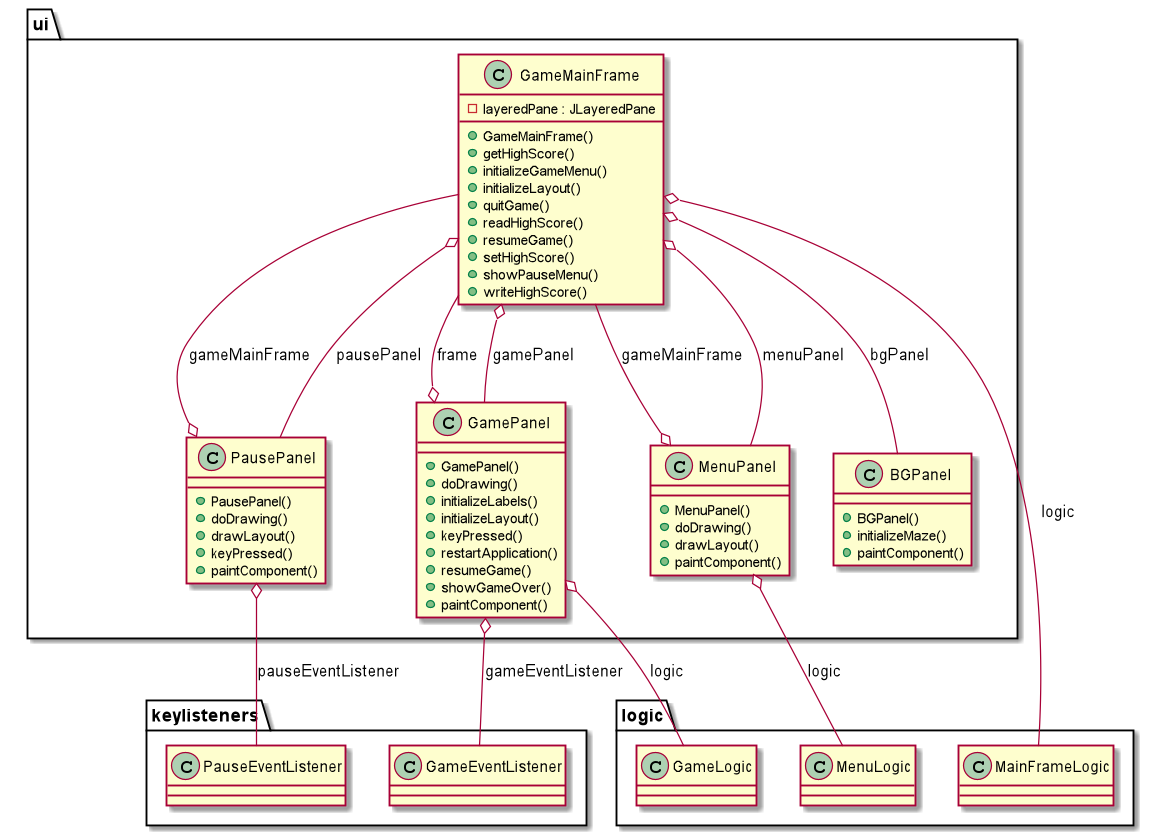
\includegraphics[width=\linewidth]{ui}
  \caption{Diagramma di classe del modulo UI}
  \label{fig:ui}
\end{figure}

% UI [end]
%-------------------------------------------

% Logic [start]
%-------------------------------------------
\section{Logic}\label{se:arch.logic}
In Fig.~\ref{fig:logic} viene illustrato il digramma di classe del modulo Logic.\newline

Le classi del “logic” si occupano dell'effettiva logica con cui le classi del “ui” mostrano le componenti e le immagini. Mentre MenuLogic, che popola la ComboBox per la scelta del labirinto nel menù principale, e MainFrameLogic, che registra il font nell’ambiente grafico e registra l’HighScore, sono solo un supporto alle loro controparti UI, GameLogic è effettivamente una delle classi più importanti dell’applicazione, in quanto si occupa di scandire i cicli effettivi Update / Repaint (nota a piè pagina: ciclo in cui vengono aggiornate le coordinate e gli stati degli oggetti, successivamente vengono stampati) del gioco e di inserire gli sprite all’interno dell’ambiente e di stabilire ciò che accade se avviene una collisione tra di essi. Mostriamo ora alcuni dei suoi metodi che vengono chiamati quando si inizia una partita:
\begin{enumerate}
 \item \textbf{GameLogic()}: Inizializza tutte le variabili necessarie al corretto funzionamento del gioco e avvia il timer principale che richiamerà periodicamente, grazie alla classe GameLoop, il metodo seguente;
 \item \textbf{doOneLoop()}: Richiede il focus della tastiera su GamePanel, richiama update() e gamePanel.repaint();
 \item \textbf{update()}: Passato il breve periodo di pausa, ordina al Pac-Man e ai fantasmi di muoversi chiamando il loro metodo move(), controlla le collisioni con checkCollision(), controlla se il livello deve terminare e sceglie quale effetto in loop riprodurre in sottofondo;
 \item \textbf{endGame()}: Chiamato se Pac-Man mangia tutte le pill, resetta il labirinto e passa al livello successivo chiamando restartLevel();
 \item \textbf{restartLevel()}: Chiamato nel caso precedente o nel caso Pac-Man perda una vita, riporta tutti i personaggi nelle loro posizioni iniziali e riavvia il timer;
 \item \textbf{restartApplication()}: Chiamato nel caso di un Game Over o se l’utente sceglie di abbandonare la partita, salva un eventuale HighScore e fa tornare il controllo al GameMainFrame.
\end{enumerate}

\begin{figure}[tb]
  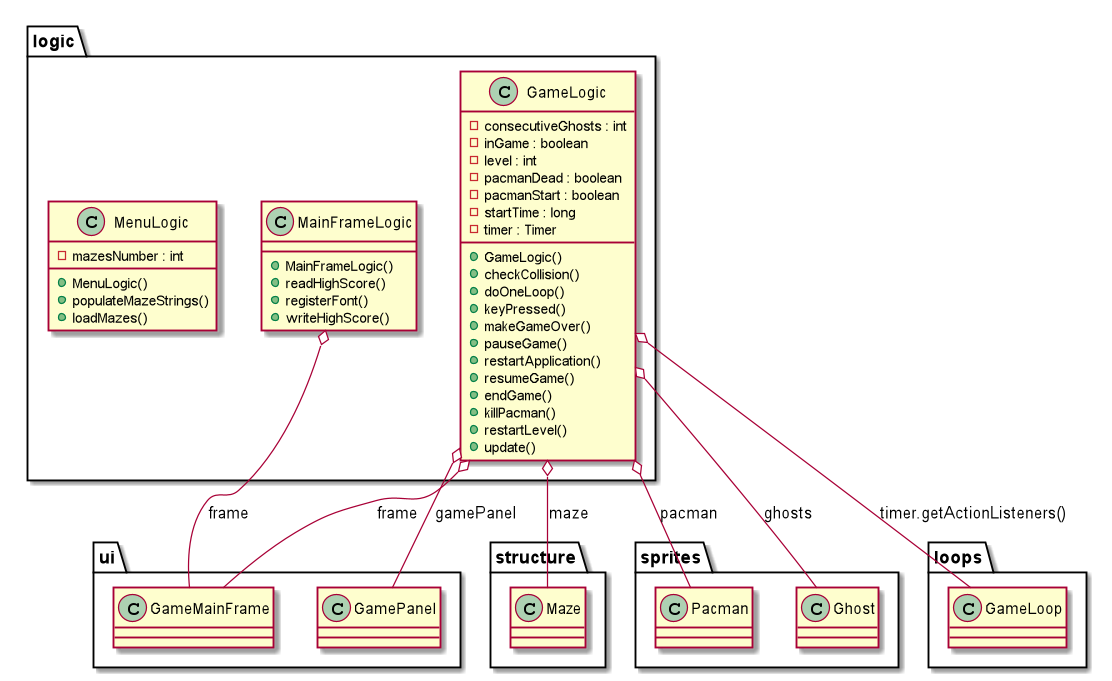
\includegraphics[width=\linewidth]{logic}
  \caption{Diagramma di classe del modulo Logic}
  \label{fig:logic}
\end{figure}

% Logic [end]
%-------------------------------------------

% Sprites [start]
%-------------------------------------------
\section{Sprites}\label{se:arch.sprites}
In Fig.~\ref{fig:sprites} viene illustrato il digramma di classe del modulo Sprites.\newline

Nel package “sprites” ogni classe estende la classe astratta Sprite e rappresenta un’entità all’interno del labirinto con tutti i valori che la descrivono (posizione, incremento del movimento, dimensioni, immagine, punti, visibilità). Le classi non astratte che estendono Sprite in maniera diretta rappresentano tutte entità fisse. Infatti, per Pill, PowerPill, Fruit e Portal, non viene definito nelle classi un vero e proprio comportamento, ma saranno Maze e il GameLogic a definire rispettivamente quando quelli potranno apparire e ciò che succede quando un’entità mobile verrà a contatto con esse tramite il suo metodo checkCollision() (es. Pac-Man entra a contatto con una PowerPill, questa sparisce e ai fantasmi viene notificata l’entrata in stato di Frightened).

Mentre gli oggetti delle classi successive, in quanto personaggi, verranno inseriti nel GameLogic direttamente come attributi, gli sprite sopracitati saranno dapprima inseriti nell’oggetto Maze, attributo in GameLogic. Ciò semplifica sia la gestione che il ripristino alla fine del livello.

Character estende Sprite ma è una classe astratta: fornisce una struttura e metodi comuni per i personaggi del labirinto come returnToSpawnPoint() per ritornare alla posizione iniziale e gli astratti move() e addFrameManager().

La prima classe ad estendere Character è Pacman: il keyListener di GamePanel gli notifica i tasti premuti dal giocatore: se sono frecce direzionali Pacman salva il codice dell’ultima premuta in keyPressed e avvia il suo timer collegato a PacmanLoop, con il metodo changeLoop() cambierà direzione in quella richiesta non appena questa sarà disponibile e fermerà il timer.

La seconda classe, seppur astratta, è Ghost: la classe implementa la logica del movimento dei fantasmi in tutti i loro stati grazie ad un sistema di coordinate target per cui sceglieranno la direzione più breve in linea d’aria senza avere la possibilità di fare dietrofront. I target sono diversi a seconda dello stato dei fantasmi:
\begin{itemize}
 \item Scatter: un lato del labirinto a seconda del fantasma;
 \item Frightened: ignora il target, il movimento è randomico;
 \item Eaten: lo Spawn Point di Blinky;
 \item Chase: dinamico durante la partita, si calcola in modo diverso per ogni fantasma con un Override del metodo setChaseTarget().
\end{itemize}
Ogni fantasma modifica dinamicamente il proprio stato grazie al suo timer, con GhostLoop che regola il cambio Chase-Scatter e decide quando terminare lo stato di Frightened, il quale si attiva col metodo di Ghost becomeFrightened(), invocato dal GameLoop nel caso di una collisione di Pac-Man con una PowerPill. In maniera analoga viene impostato lo stato di Eaten.
Tra i quattro fantasmi l’unica differenza considerevole è la presenza di un riferimento a Blinky in Inky, il quale ha bisogno di ottenere dinamicamente sia le coordinate di Pacman (come gli altri) che di Blinky per poter calcolare il suo Chase Target.

Tutti i Character controllano la possibilità di muoversi avanti o di cambiare direzione tramite i metodi messi a disposizione dalla classe statica MazeManager che vedremo in seguito.


\begin{figure}[p]
\begin{center}
 \centerline{ 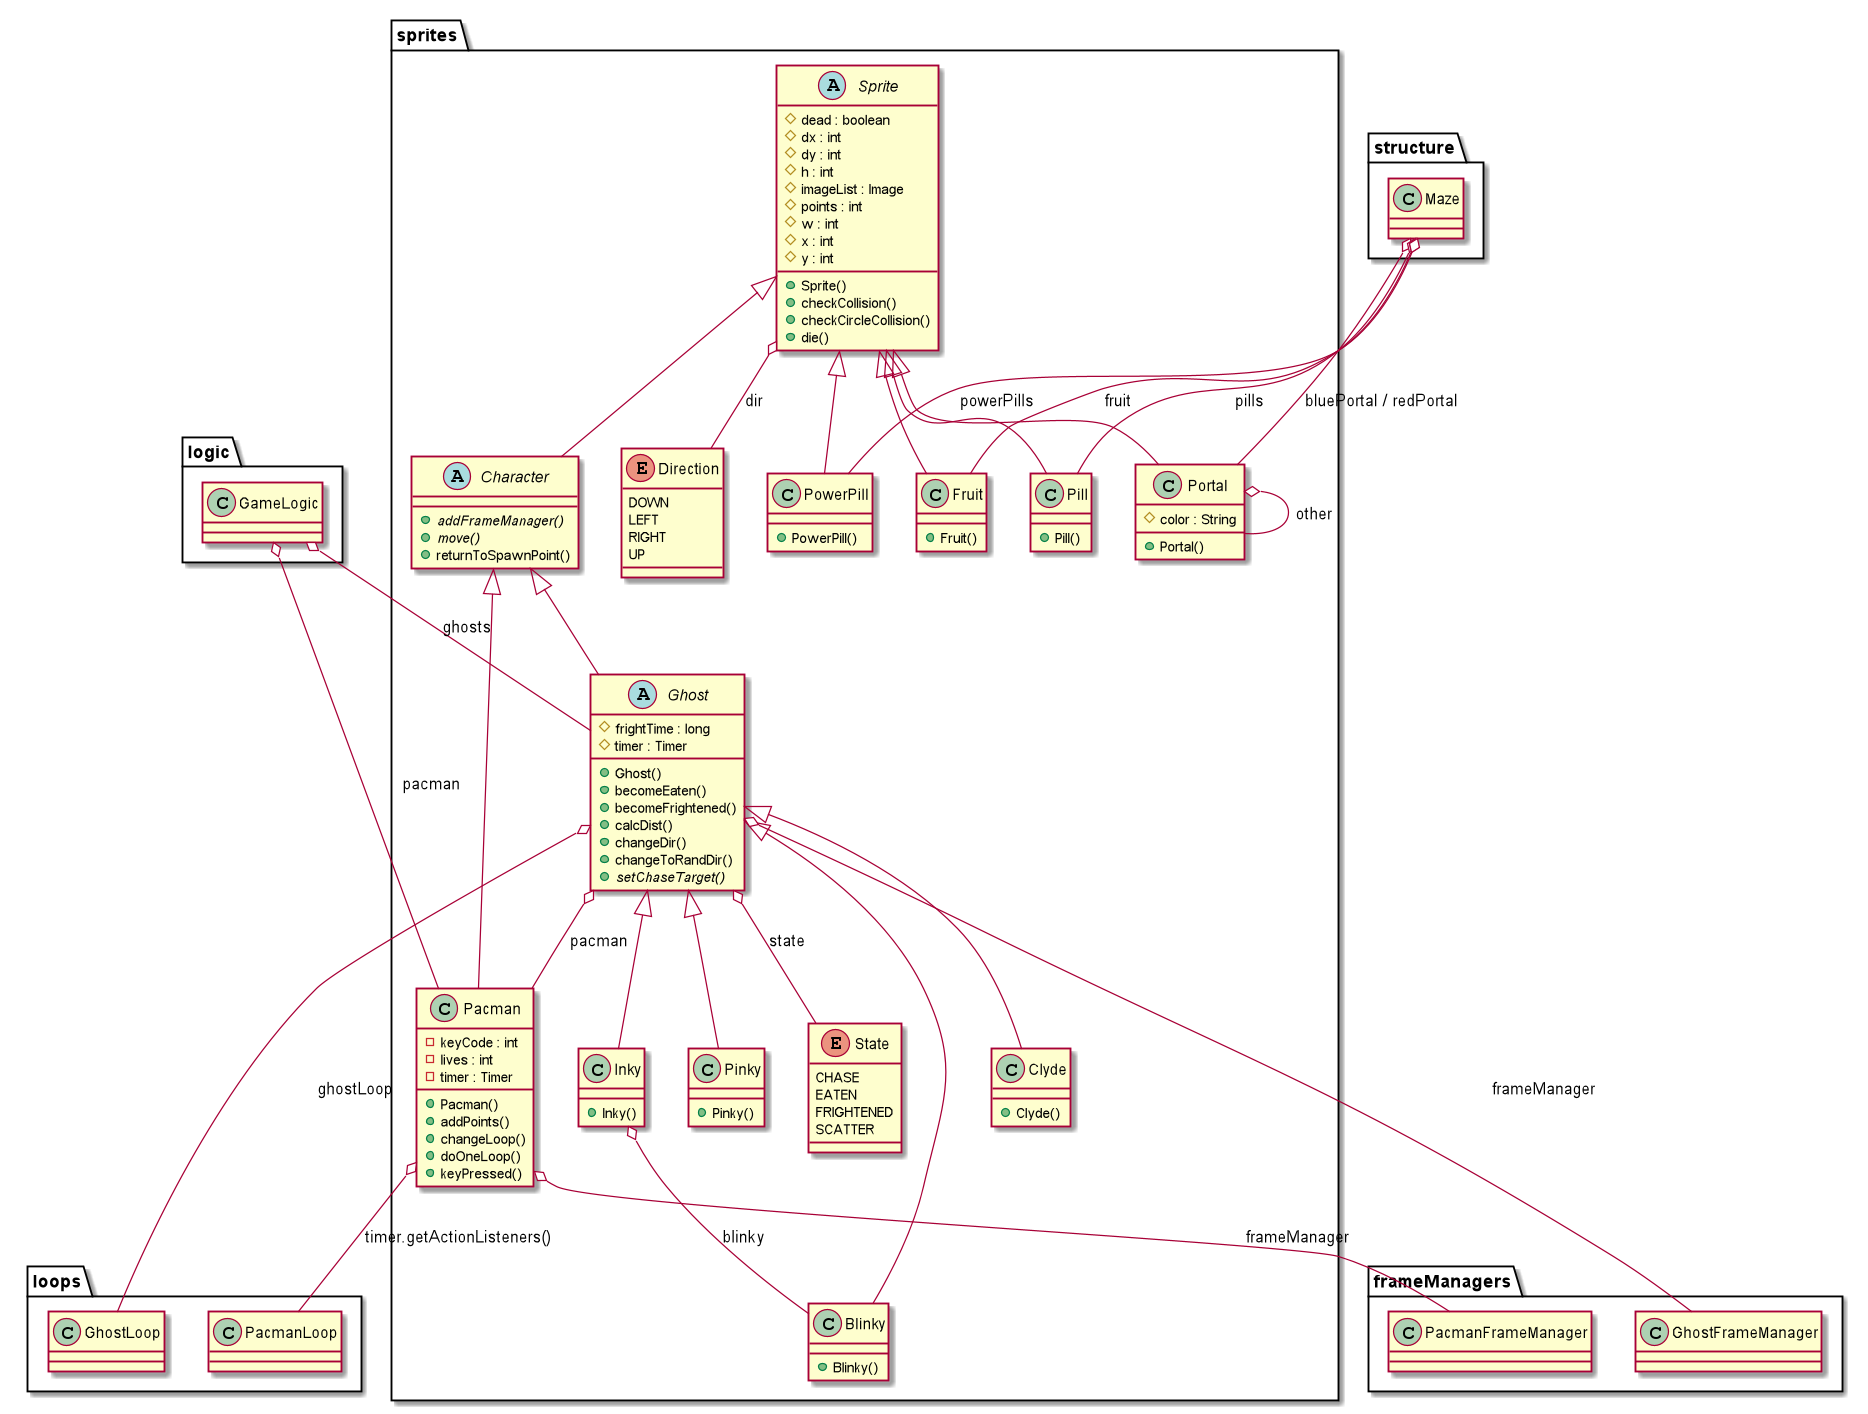
\includegraphics[width=20cm]{sprites}}
\end{center}
  \caption{Diagramma di classe del modulo Sprites}
  \label{fig:sprites}
\end{figure}

\newpage

% Sprites [end]
%-------------------------------------------

% Structure [start]
%-------------------------------------------
\section{Structure}\label{se:arch.structure}
In Fig.~\ref{fig:structure} viene illustrato il digramma di classe del modulo Structure.\newline

Il package structure ci permette di creare la struttura del labirinto partendo da un file txt nel File System e di gestire il movimento dei personaggi al suo interno e gli elementi di gioco fissi con cui i primi possono interagire.
La prima classe ad entrare in gioco è la statica MazeManager, la quale legge il file di testo (una matrice di caratteri che definiremo in seguito) richiesto e restituisce una matrice di char da cui il BGPanel ricaverà un labirinto da poter mostrare con createMaze(). Con populateMaze() invece popolerà il labirinto di elementi di gioco e restituirà l’oggetto del Maze al GameLogic (che lo richiamerà per ripopolarlo ogni volta che si vorrà passare al livello successivo).

Troviamo poi metodi statici la cui utilità è quella di permettere ai Characters di generarsi e muoversi nel labirinto con le dovute restrizioni:
\begin{itemize}
 \item \textbf{canIMove()}: I Character, essendo grossi esattamente le dimensioni di un blocco, potranno muoversi esclusivamente quando la loro coordinate saranno entrambe multipli di tale dimensione, questo metodo controlla ciò e restituisce un esito booleano.
 \item \textbf{checkEmpty()}: Date le coordinate e la direzione di un Character, controlliamo che il prossimo blocco in quella direzione sia vuoto o sia un muro.
 \item \textbf{getObjCoord()}': Dato un char, restituisce la coordinata di dove si trova nella struttura labirintica (es. lo Spawn Point di Pac-Man è rappresentato con “S”).
 \item \textbf{whichBlock()}: date le coordinate di un blocco del labirinto, restituisce il char corrispondente a quel blocco.
\end{itemize}

La classe Maze funge da struttura dati su cui memorizzare la matrice di char che rappresenta il labirinto e tutti gli Sprite statici (non Character). L’unico sprite per cui implementiamo in questa classe un criterio di restituzione è Fruit.
La classe Coordinate serve solo per memorizzare coppie di interi per utilizzarle nelle altre classi.\newpage


\begin{figure}[tb]
\begin{center}
  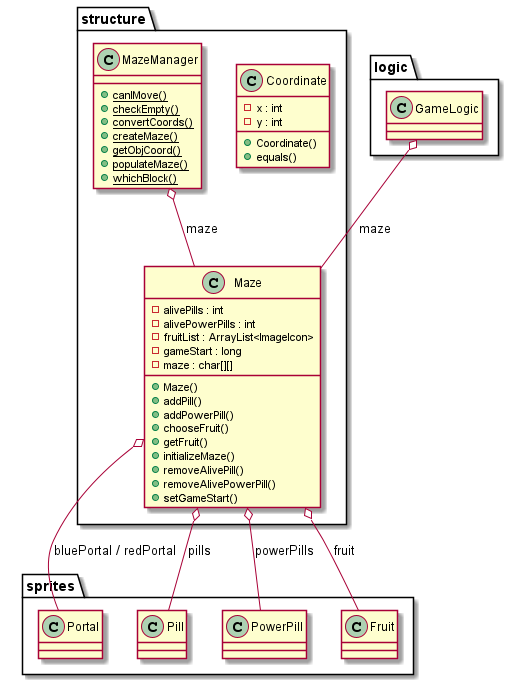
\includegraphics[width=10cm]{structure}
\end{center}
  \caption{Diagramma di classe del modulo Structure}
  \label{fig:structure}
\end{figure}


% Structure [end]
%-------------------------------------------

% Loops [start]
%-------------------------------------------
\section{Loops}\label{se:arch.loops}
In Fig.~\ref{fig:loops} viene illustrato il digramma di classe del modulo Loops.\newline

Nel package loops sono contenute le classi che vengono richiamate periodicamente nelle classi in cui è contenuto il loro riferimento, con l’ausilio di un timer. PacmanLoop e GameLoop richiamano il metodo doOneLoop() rispettivamente di PacmanLogic e GameLogic di cui si è già trattato in precedenza.

GhostLoop, d’altro canto, è sicuramente la classe più corposa e complessa delle tre, in quanto tiene traccia dei cambiamenti di stato dei fantasmi e dei periodi in cui ogni stato deve essere mantenuto: tiene infatti conto dei secondi rimanenti negli stati di Chase/Scatter anche una volta che si entra negli stati di Frigtened/Eaten.

\begin{figure}[tb]
\begin{center}
  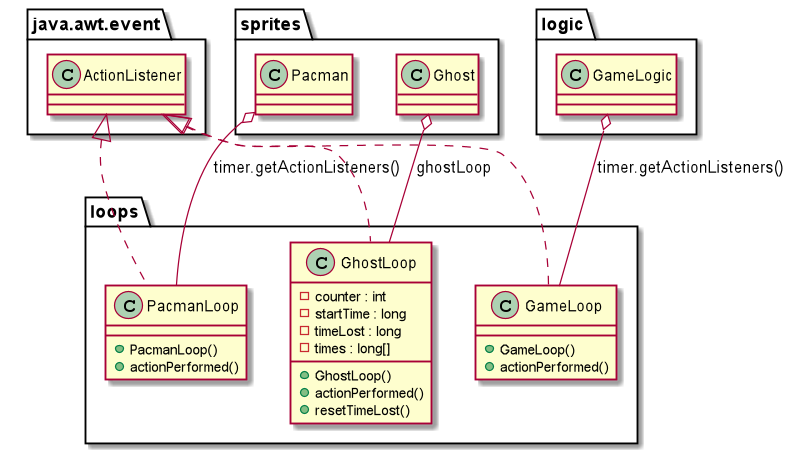
\includegraphics[width=15cm]{loops}
\end{center}
  \caption{Diagramma di classe del modulo Loops}
  \label{fig:loops}
\end{figure}

% Loops [end]
%-------------------------------------------

% FrameManagers [start]
%-------------------------------------------
\section{FrameManagers}\label{se:arch.frameManagers}
In Fig.~\ref{fig:frameManagers} viene illustrato il digramma di classe del modulo FrameManagers.\newline

FrameManager permette di implementare effetti di animazione dei personaggi. Infatti i Character, a ogni chiamata del loro metodo move() andranno a richiamare getNextFrame(), il quale, a seconda del caso e sulla base del frame precedente, è in grado di restituire una nuova immagine da applicare allo sprite, che verrà poi stampata su GamePanel. 
PacmanFrameManager  e GhostFrameManager sono delle specializzazioni che implementano rispettivamente, l’animazione della morte del Pacman e i fantasmi in stati di Frightened e Eaten. 
Invece di inserire negli ArrayList immagini identiche più volte, abbiamo implementato un valore di ritardo in modo da restituire ripetutamente lo stesso frame, al fine di garantire un movimento più fluido. 
Data la ciclicità delle animazioni - eccetto quella della morte del Pacman - gli ArrayList di ImageIcon vengono fatti scorrere al dritto e al rovescio tramite l’utilizzo della booleana forward.

\begin{figure}[tb]
\begin{center}
  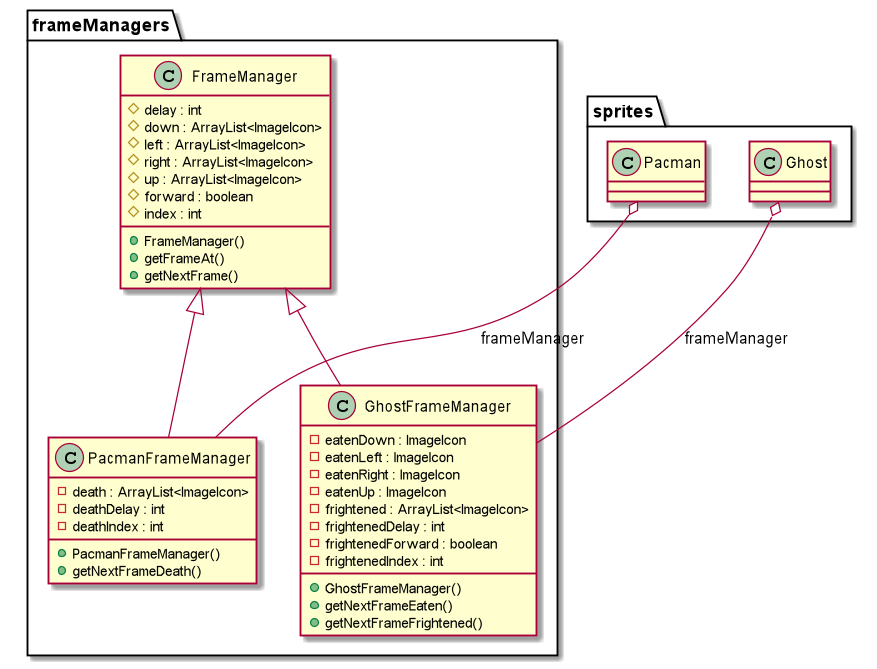
\includegraphics[width=15cm]{frameManagers}
\end{center}
  \caption{Diagramma di classe del modulo FrameManagers}
  \label{fig:frameManagers}
\end{figure}

% FrameManagers [end]
%-------------------------------------------

% KeyListeners [start]
%-------------------------------------------
\section{KeyListeners}\label{se:arch.keyListeners}
In Fig.~\ref{fig:keyListeners} viene illustrato il digramma di classe del modulo KeyListeners.\newline

Semplici KeyListener aggiunti a GamePanel, per inviare i comandi a Pac-Man o mettere pausa con il tasto Invio, e PausePanel, per uscire dalla pausa sempre con Invio. \newpage

\begin{figure}[tb]
\begin{center}
  \includegraphics[width=12cm]{keyListeners}
\end{center}
  \caption{Diagramma di classe del modulo KeyListeners}
  \label{fig:keyListeners}
\end{figure}

% KeyListeners [end]
%-------------------------------------------

% Sound [start]
%-------------------------------------------
\section{Sound}\label{se:arch.sound}
In Fig.~\ref{fig:sound} viene illustrato il digramma di classe del modulo Sound.\newline

Il Package sound mette a disposizione metodi per l’avvio di effetti sonori e sottofondi musicali, permette all’utente di disattivarli e attivarli a piacimento e, tramite SoundFactory, gestisce il caricamento dal File System e la gestione dello stream audio.
Il SoundPlayer tiene inoltre traccia di tutti gli effetti musicali in riproduzione e gli effetti sonori in loop in quel dato istante in modo da evitare sovrapposizione con conseguente distorsione.
Per riprodurre una Clip, SoundPlayer utilizza un oggetto di classe SoundFactory, che richiama dapprima il metodo chooseSound() per creare un SoundClip dato l’elemento corrispondente nell’Enum Sound, contenente i nomi dei file audio. L’oggetto creato viene dato in input a playSound(), che apre lo stream e vi riproduce la Clip.\newpage

\begin{figure}[tb]
\begin{center}
  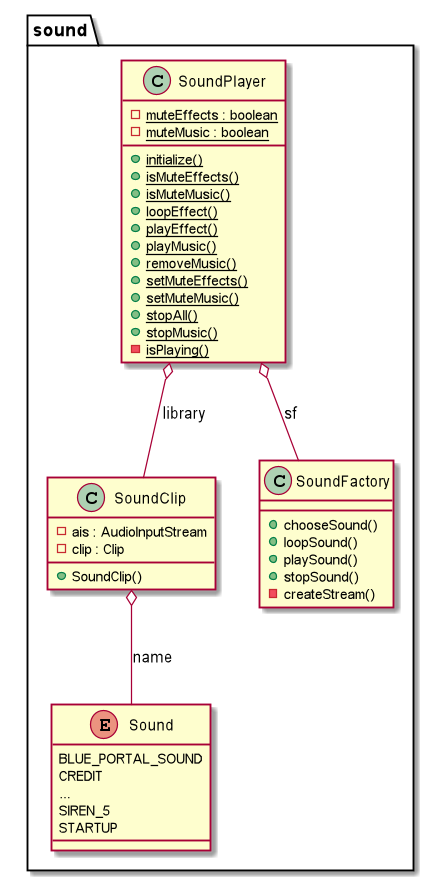
\includegraphics[width=0.5\linewidth]{sound}
\end{center}
  \caption{Diagramma di classe del modulo Sound}
  \label{fig:sound}
\end{figure}

% Sound [end]
%-------------------------------------------

% Image [start]
%-------------------------------------------
\section{Image}\label{se:arch.image}
In Fig.~\ref{fig:image} viene illustrato il digramma di classe del modulo Image.\newline

ImageFactory si occupa semplicemente di creare una ImageIcon dato un elemento dell’Enum ImageList, che corrisponde a un file su disco.

\begin{figure}[tb]
\begin{center}
  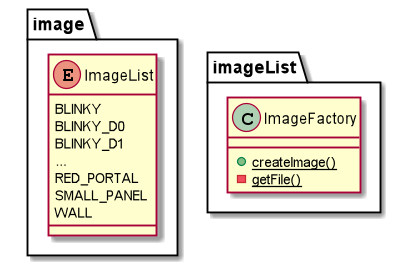
\includegraphics[width=15cm]{image}
\end{center}
  \caption{Diagramma di classe del modulo Image}
  \label{fig:image}
\end{figure}

% Image [end]
%-------------------------------------------




% Problemi Riscontrati [start]
%-------------------------------------------
\section{Problemi Riscontrati}\label{ch:proris}
% Problemi Riscontrati [end]
Nella creazione dell’applicazione non si sono riscontrati particolari problemi per quanto riguarda la gestione del movimento dei fantasmi o del Pacman o nella creazione del labirinto. 
Sicuramente la modalità con cui i fantasmi raggiungono il target non è impeccabile, in quanto esistono molte situazioni in cui il fantasma, calcolando il percorso più breve in linea d’aria senza tener conto delle mura del labirinto, sarà portato a prendere direzioni non sempre precise. Nonostante ciò, questa imprecisione dell’algoritmo non va ad influenzare negativamente l’esperienza di gioco, facilitando invece l’esperienza.

Una difficoltà riscontrata nello scegliere il target di movimento per i fantasmi è stata nella scelta del target da raggiungere dai fantasmi in stato di Eaten. Abbiamo deciso di scegliere per tutti e quattro i fantasmi lo spawn point di Blinky poichè, essendo ubicato nella casella più esterna della casetta, dava meno problemi al fantasma in Eaten di poter rinascere.

La logica di gestione degli elementi statici del labirinto non è complessa, ma un problema riscontrato spesso è stato l’impossibilità del Pacman di riuscire a mangiare l’ultima pallina del labirinto. Questo perchè il gioco terminava appena Pacman collideva con l’ultima pallina e quindi tutte le animazioni si fermavano ancor prima che il Pacman riuscisse a dare l’impressione al giocatore di averla mangiata. Per ovviare a questo abbiamo implementato un ritardo di 50 millisecondi prima che il gioco terminasse definitivamente.

Proprio alla fine del gioco, esaurite tutte le vite, nella creazione della Label per il GameOver, essendo che il ciclo update/repaint viene fermato, non veniva mostrata su schermo l’opportuna dicitura. Pertanto abbiamo invocato il metodo paintImmediately() di JLabel che ci ha permesso di stampare “GAME OVER” senza bisogno che il metodo repaint() di GamePanel entrasse in azione.
Inoltre, a livello dell’esperienza di gioco, è stato complesso rendere fluido il movimento del Pacman con i fantasmi all’interno del labirinto, in quanto spesso sono sorti problemi di accelerazione e decelerazione eccessiva rispetto alla velocità desiderata. Tale problema risulta essere presente, sulla base di svariate prove, se il calcolatore sul quale si gioca possiede una scheda grafica dotata di aggiornamento verticale sincronizzato (VSYNC). Un’altra motivazione potrebbe essere la presenza di un componente grafico sgradito alla nostra applicazione nel nuovo aggiornamento di Windows 10 (2004), in quanto solo dopo averlo eseguito su due calcolatori differenti sono stati riscontrati problemi di questo tipo (anche disattivando il VSYNC). Nonostante queste plausibili motivazioni, vi potrebbero essere anche altri fattori di cui però non siamo riusciti a venire a conoscenza.

Infine, ciò che più di tutti ha reso complessa la scrittura del gioco, è stata la gestione dei numerosi suoni ed effetti presenti continuamente in sottofondo. 
A partire dal fatto che inizialmente, per riavviare il gioco non appena Pacman era morto, oppure per ricominciare il livello una volta che Pacman è stato preso da fantasma, il JFrame si chiudeva e riapriva all’istante, lasciando così aperti gli stream dei suoni, che andando avanti con il gioco, causava sovrapposizione tra gli effetti e anche il suono stesso veniva distorto. Perciò abbiamo deciso di utilizzare sempre lo stesso JFrame, e di far ripartire il gioco togliendo dal layeredPane il BGPanel per il labirinto, e il Gamepanel per rimuovere pillole e tutto il resto degli elementi, per poi andare a reinserire tali strati senza bisogno di ricreare il JFrame. Inoltre necessaria è stata la creazione della classe SoundClip che permette oltretutto la chiusura degli stream audio una volta terminato il loro utilizzo, così da evitare l’insorgere di eventuali altri problemi.

% Problemi Riscontrati [stop]
%-------------------------------------------
%%%%%%%%%%%%%%%%%%%%%%%%%%
%     Progetto [end]     %
%%%%%%%%%%%%%%%%%%%%%%%%%%



%%%%%%%%%%%%%%%%%%%%%%%%%%%%%%%%%%%%%%%%%%%%%%%%%
%     Conclusioni e sviluppi futuri [start]     %
%%%%%%%%%%%%%%%%%%%%%%%%%%%%%%%%%%%%%%%%%%%%%%%%%
\chapter{Conclusioni e sviluppi futuri}\label{ch:conc-svil-fut}
\lipsum[29-30]
%%%%%%%%%%%%%%%%%%%%%%%%%%%%%%%%%%%%%%%%%%%%%%%
%     Conclusioni e sviluppi futuri [end]     %
%%%%%%%%%%%%%%%%%%%%%%%%%%%%%%%%%%%%%%%%%%%%%%%



%%%%%%%%%%%%%%%%%%%%%%%%%%%%%%%%%%%%%%%%%%%%%
%     Bibliografia e Sitografia [start]     %
%                with BibTeX                %
%%%%%%%%%%%%%%%%%%%%%%%%%%%%%%%%%%%%%%%%%%%%%
\bibliographystyle{plain}
\bibliography{bibliografia}
% inserire i riferimenti bibliografici nel file 'bibliografia.bib'
%%%%%%%%%%%%%%%%%%%%%%%%%%%%%%%%%%%%%%%%%%%
%     Bibliografia e Sitografia [end]     %
%                with BibTeX              %
%%%%%%%%%%%%%%%%%%%%%%%%%%%%%%%%%%%%%%%%%%%

\end{document}
%%%%%%%%%%%%%%%%%%%%%%%%%%%%%%%%
%                              %
%     Begin Docuemnt [end]     %
%                              %
%%%%%%%%%%%%%%%%%%%%%%%%%%%%%%%%